\chapter{RÉSULTAT ET DISCUSSIONS}
Ce chapitre se concentre sur l’analyse des résultats de prédiction obtenus après l’application des méthodes de machine learning aux données climatiques et aux cas antérieurs de Chikungunya dans trois pays : le \textbf{Tchad}, le \textbf{Brésil} et le \textbf{Paraguay}. L’objectif est de présenter en détail les résultats, de proposer une discussion approfondie, et d’identifier les éventuelles lacunes ou limitations.

\section{Méthode de Validation Croisée (Entraînement et Test)}
L'ensemble de données, composé de 366 instances pour le \textbf{Tchad} et de 1826 instances pour le \textbf{Brésil} et le \textbf{Paraguay}, comprenant des données climatiques et des informations sur les cas de Chikungunya, a été divisé en deux parties pour l’apprentissage. Tout d’abord, les données ont été mélangées, puis elles ont été séparées en deux ensembles : 80 \% des données ont été utilisées pour l’entraînement (ensemble d’apprentissage) et 20 \% ont été réservées pour les tests (ensemble de test).

\section{Choix des Hyperparamètres des Modèles d'Ensemble}
Les hyperparamètres des modèles utilisés pour déterminer leurs performances sont détaillés ci-dessous.

\subsection{Cas du Random Forest Regressor}
Cette section détaille les choix des hyperparamètres spécifiques pour le \textbf{Random Forest Regressor} et leur impact sur la précision des prédictions. Ces hyperparamètres ont été ajustés à l’aide de la méthode de \textbf{recherche en grille} (\textbf{Grid Search}) afin d’optimiser les performances du modèle illustré dans le tableau \ref{tab:grid-search-rf}.

\begin{table}[!hbt]
	\centering
	\caption{Description des hyperparamètres optimisés pour le Random Forest Regressor avec GridSearch}
	\label{tab:grid-search-rf}
	\begin{tabular}{|c|c|c|c|c|}
		\hline
		& \multicolumn{4}{c|}{Hyperparamètres} \\
		\hline
		Pays & \textsf{n\_estimators} & \textsf{max\_depth} & \textsf{min\_samples\_leaf} & \textsf{min\_samples\_split} \\
		\hline
		Tchad & 200 & 10 & 2 & 2 \\
		\hline
		Brésil & 200 & 20 & 2 & 2 \\
		\hline
		Paraguay & 200 & None & 1 & 5 \\
		\hline
	\end{tabular}
\end{table}

Les hyperparamètres utilisés pour le \textbf{Random Forest Regressor} sont les suivants :
\begin{itemize}
	\item \textbf{n\_estimators} : Le nombre d'arbres dans la forêt. Un nombre plus élevé d'arbres peut améliorer la performance, mais augmente aussi le temps de calcul.
	\item \textbf{max\_depth} : La profondeur maximale des arbres. Une profondeur plus grande permet au modèle de capturer plus de complexité, mais risque de surapprendre (overfitting).
	\item \textbf{min\_samples\_leaf} : Le nombre minimum d'échantillons requis pour être dans une feuille. Un nombre plus élevé peut entraîner un modèle plus simple et réduire le surapprentissage.
	\item \textbf{min\_samples\_split} : Le nombre minimum d'échantillons requis pour diviser un nœud interne. Un nombre plus élevé peut rendre le modèle moins sensible au bruit.
\end{itemize}

\subsection{Cas du XGBoost Regressor}
Cette section présente les hyperparamètres choisis pour le \textbf{XGBoost Regressor} et leur impact sur la précision des prédictions. Ces hyperparamètres ont également été ajustés à l’aide de la méthode de \textbf{recherche en grille} (\textbf{Grid Search}) afin d’optimiser les performances du modèle illustré dans le tableau \ref{tab:grid-search-xb}.

\begin{table}[!hbt]
	\centering
	\caption{Description des hyperparamètres optimisés pour le XGBoost Regressor avec GridSearch}
	\label{tab:grid-search-xb}
	\begin{tabular}{|c|c|c|c|c|}
		\hline
		& \multicolumn{4}{c|}{Hyperparamètres} \\
		\hline
		Pays & \textsf{n\_estimators} & \textsf{max\_depth} & \textsf{subsample} & \textsf{learning\_rate} \\
		\hline
		Tchad & 300 & 5 & 0.8 & 0.2 \\
		\hline
		Brésil & 100 & 5 & 1.0 & 0.2 \\
		\hline
		Paraguay & 100 & 7 & 0.1 & 0.2 \\
		\hline
	\end{tabular}
\end{table}

Les hyperparamètres utilisés pour le \textbf{XGBoost Regressor} sont les suivants :
\begin{itemize}
	\item \textbf{n\_estimators} : Le nombre d'arbres dans la forêt.
	\item \textbf{max\_depth} : La profondeur maximale des arbres. Comme pour le Random Forest, une plus grande profondeur peut capturer plus de complexité, mais risque de surapprentissage.
	\item \textbf{subsample} : La proportion d'échantillons utilisés pour entraîner chaque arbre. Une valeur inférieure à 1.0 réduit le surapprentissage en introduisant plus de diversité dans les arbres.
	\item \textsf{learning\_rate} : Le taux d'apprentissage, qui contrôle la contribution de chaque modèle supplémentaire. Un taux plus bas nécessite plus d'estimators pour converger, mais peut conduire à une meilleure généralisation.
\end{itemize}

\section{Résultats obtenus par nos modèles}
Cette section, nous exposons nos résultats à travers un tableau, suivi d’une discussion approfondie. Par la suite, nous illustrons les diverses mesures de performance à l’aide de graphiques variés.
\subsection{Tableau des performance de nos modèles}
Le tableau~\ref{tab:performance} ci-dessous illustre les métriques d’évaluation des résultats de nos travaux.

Les résultats obtenus montrent que le \textit{modèle d'ensemble}, en particulier le \textbf{Voting Regressor}, a globalement surpassé les autres modèles en termes de précision. Il a permis de réduire les erreurs (\textbf{MAE} et \textbf{RMSE}) et d'augmenter le score R\textsuperscript{2}, indiquant une meilleure explication de la variance des données.

Pour le \textbf{Paraguay}, le \textbf{Voting Regressor} a obtenu un RMSE  faible (\textbf{62.25}) et le meilleur score R\textsuperscript{2} (\textbf{0.5957}), surpassant les modèles LinearRegressor et XGBoostRegressor.

Au \textbf{Brésil}, bien que le modèle XgboostRegressor ait montré de très bonnes performances (RMSE de\textbf{1459.15} et R\textsuperscript{2} de \textbf{0.65}), le \textbf{Voting Regressor} a réussi à obtenir des résultats comparables avec un RMSE particulièrement bas de \textbf{1387.23}.

Pour le \textbf{Tchad}, les performances des modèles étaient globalement plus faibles, mais le \textbf{Voting Regressor} a tout de même montré une légère amélioration par rapport aux autres modèles, bien que le score R\textsuperscript{2} reste faible (\textbf{0.282}).

En conclusion, les modèles d'ensemble, et particulièrement le \textbf{Voting Regressor}, a révélés être les plus performants pour prédire les cas de Chikungunya dans les trois pays étudiés.Toutefois, avec des prédictions plus fiables pour le \textbf{Brésil} et le \textbf{Paraguay} que pour le Tchad, ce qui est dû à la quantité des données disponibles pour ce pays là.

\begin{table}[h!]
	\centering
	\caption{Métriques de performance des modèles (MAE, RMSE, R² Score) pour le Brésil, le Tchad et le Paraguay}
	\begin{tabular}{|c|c|c|c|c|}
		
		\hline
		\textbf{Pays} & \textbf{Modèle} & \textbf{MAE} & \textbf{RMSE} & \textbf{R² Score} \\ 
		\hline
		\multirow{4}{*}{Brésil} & Linear Regression & 1178.99 & 1591.25 & 0.447 \\ 
		& Random Forest Regressor & 897.17  & 1477.20 & 0.523 \\ 
		& XGBoost Regressor & 827.16  & 1459.15 & 0.535 \\ 
		& \textbf{Voting Regressor} & \textbf{840.14}  & \textbf{1387.23} & \textbf{0.65} \\ 
		\hline
		\multirow{4}{*}{Tchad}  & Linear Regression & 56.06   & 98.34   & 0.198 \\ 
		& Random Forest Regressor & 47.81   & 80.90   & 0.457 \\ 
		& XGBoost Regressor & 55.17   & 101.13  & 0.152 \\ 
		& \textbf{Voting Regressor} & \textbf{50.52}   & \textbf{93.02}   & \textbf{0.282} \\ 
		\hline
		\multirow{4}{*}{Paraguay} & Linear Regression & 67.15   & 84.68   & 0.332 \\ 
		& Random Forest Regressor & 35.31   & 61.28   & 0.650 \\ 
		& XGBoost Regressor & 40.32   & 71.95   & 0.517 \\ 
		& \textbf{Voting Regressor} & \textbf{40.37}   & \textbf{62.25}   & \textbf{0.59,97} \\ 
		\hline
	\end{tabular}
	
\end{table}

\subsection{Performance en RMSE , R2 Score et MAE}
La figure \ref{fig:metriccomparaison} montre en termes de RMSE et de coefficient de détermination R2, le niveau de performance de chacun des modèles.
\begin{figure}[h!]
	\centering
	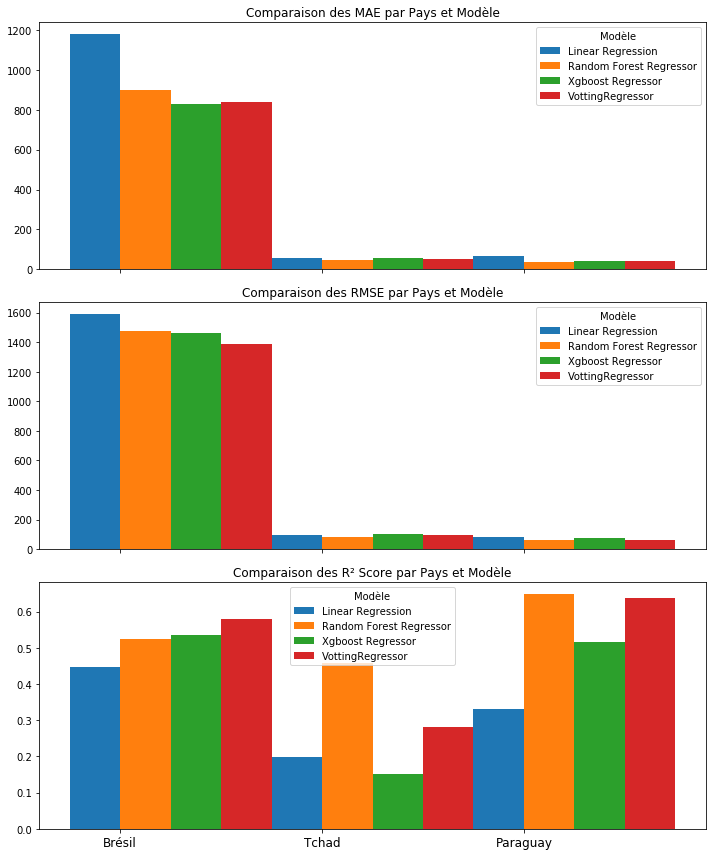
\includegraphics[width=0.8\linewidth]{images/metric_comparaison}
	\caption{Comparaison performance}
	\label{fig:metriccomparaison}
\end{figure}
\newpage
\subsection{Prédiction}
Ci-dessous les prédiction des test dans chaque pays pour le modèle d'ensemble (\textbf{VotingRegressor})
\subsubsection{Pour le Brésil}
La figure \ref{fig:predictionbresil} illustre la phase de prédiction du chikungunya au brésil. 
\begin{figure}[h!]
	\centering
	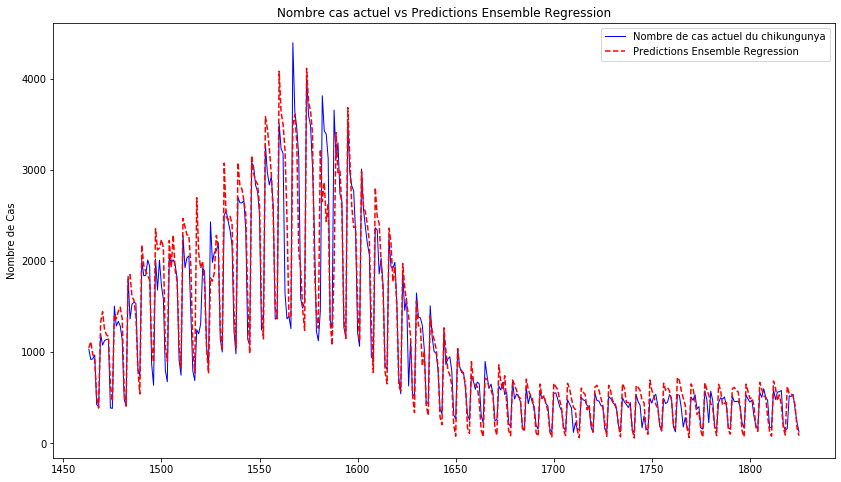
\includegraphics[width=1\linewidth]{images/prediction_bresil}
	\caption{Prédiction Brésil}
	\label{fig:predictionbresil}
\end{figure}

\subsubsection{Pour le Tchad}
La figure \ref{fig:predictionchad} illustre la phase de prédiction du chikungunya au Tchad. 
\begin{figure}[h!]
	\centering
	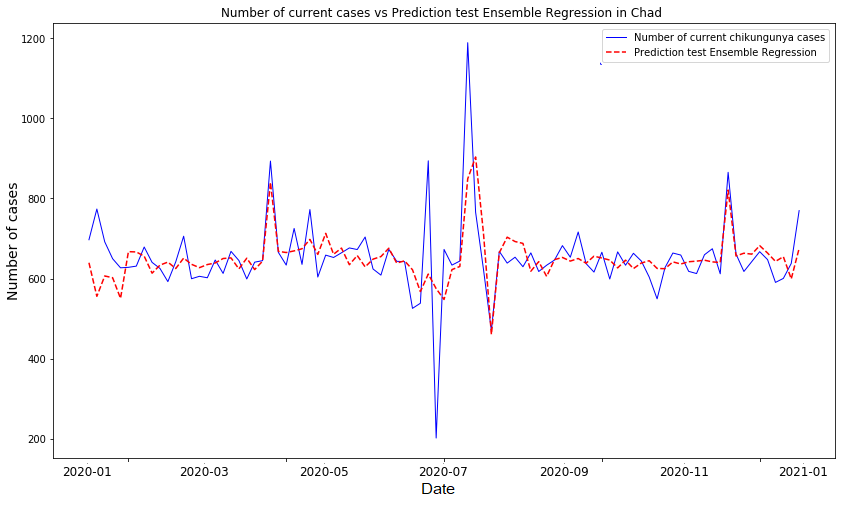
\includegraphics[width=0.85\linewidth]{images/prediction_chad}
	\caption{Prédiction Tchad}
	\label{fig:predictionchad}
\end{figure}
\subsubsection{Pour le Paraguay}
La figure \ref{fig:predictionparaguay} illustre la phase de prédiction du chikungunya au paraguay. 
\begin{figure}[h!]
	\centering
	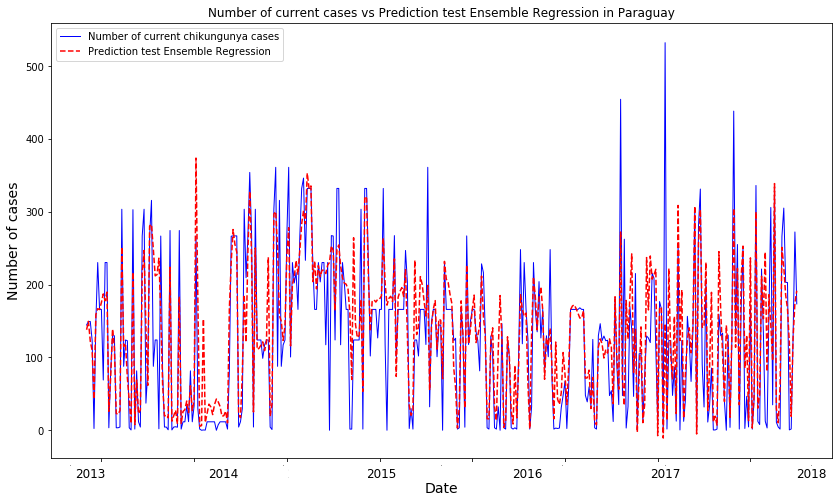
\includegraphics[width=0.85\linewidth]{images/prediction_paraguay}
	\caption{Prédiction Paraguay}
	\label{fig:predictionparaguay}
\end{figure}
\subsection{\textquotedblleft Forecasting\textquotedblright de la maladie au Brésil (3 ans)}
La figure \ref{fig:prediction} illustre la phase de prédiction du chikungunya au brésil. 
\begin{figure}[h!]
	\centering
	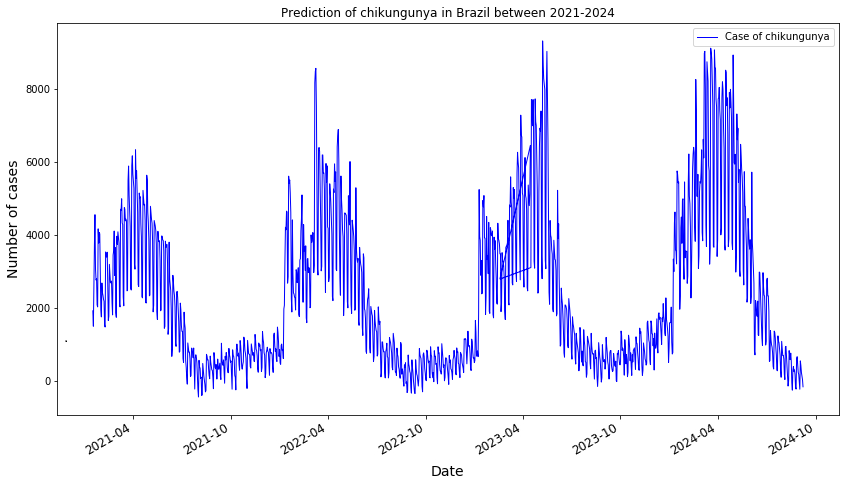
\includegraphics[width=0.85\linewidth]{images/pred_chikv}
	\caption{Prédiction Brésil}
	\label{fig:prediction}
\end{figure}
\newpage
\section{Discussion}

Les résultats obtenus dans notre étude montrent une performance compétitive des modèles de régression appliqués aux données climatiques et épidémiologiques de la Chikungunya. En particulier, notre modèle d'ensemble \textit{Voting Regressor}, qui combine les prédictions des modèles \textit{Linear Regressor}, \textit{RandomForest Regressor}, et \textit{XGBoost Regressor}, a affiché des performances globalement supérieures aux autres modèles individuels, avec un \textbf{MAE} minimal et un \textbf{RMSE} relativement bas.

Dans le cas du \textbf{Paraguay}, le \textit{Voting Regressor} a atteint un \textbf{MAE} de \textbf{40.37}, soit une amélioration par rapport au \textit{LinearRegressor}  qui affichent des \textbf{MAE} de \textbf{67.15} . Le RMSE du \textit{Voting Regressor} est de 62.25, indiquant une bonne capacité de prédiction malgré la complexité des données épidémiologiques et climatiques. Le score R² de \textbf{0.59 } montre que ce modèle explique environ 60 \% de la variance des données pour cette région, bien évidement que les techniques de \textbf{data augmentation} et du \textbf{KNNimputer} ont été d'une importance crucial sur ces résultats.

Pour le \textbf{Brésil}, le \textit{Voting Regressor} a montré une robustesse similaire avec un score R² de \textbf{0.65}, ce qui est supérieur à celui du \textit{RandomForestRegressor} et du \textit{XGBoostRegressor} et un \textbf{RMSE} minimale (1387.23) comparé aux autres modèles. Cela suggère que le \textit{Voting Regressor} parvient à combiner les forces de chaque modèle pour fournir des prédictions plus équilibrées.

Au \textbf{Tchad}, bien que les performances générales des modèles soient moins élevées, le \textit{Voting Regressor} reste le modèle le plus performant avec un \textbf{MAE} de \textbf{50.52} et un RMSE de \textbf{93.02}. Le score R² de \textbf{0.282} est le plus élevé parmi les modèles testés pour cette région, indiquant que ce modèle capture mieux la variance des données malgré des difficultés apparentes liées à la la quantité des données disponibles pour cette région, bien évidement que les techniques de \textbf{data augmentation} et du \textbf{KNNimputer} ont été d'une importance crucial sur ces résultats.

Dans notre contexte, l'imprécision observée dans certaines régions, comme au Tchad, pourrait être due à un manque de prédicteurs ou de variables explicatives dans le modèle, ce qui suggère qu'une exploration plus approfondie des facteurs climatiques et épidémiologiques est nécessaire. De plus, l'impact des variables climatiques telles que la \textbf{température} et l'\textbf{humidité} mérite une attention particulière. Il a été observé, par exemple, qu'une augmentation de la température pourrait être associée à une diminution des cas de Chikungunya, tandis que l'\textbf{humidité} semble accroître ces cas. Ce genre de corrélations, bien que contre-intuitives, pourrait fournir des pistes intéressantes pour affiner les modèles prédictifs.